\documentclass[../main.tex]{subfiles}


\begin{document}
\subsection{VM cliente Linux}\label{sec:cliente_vmlinux}
\begin{table}[htbp]
  \centering
  \begin{tabular}{rl}
    
    hostname:&Node02\\
    Sistema Operativo:&Centos 8\\
  \end{tabular}
\end{table}

\subsection{Tarjeta de red}\label{sec:ctr}
\begin{table}[htbp]
  \centering
  \begin{tabular}{rl}
    
    IP:&$192.168.100.28/24$\\
    Puerta de Enlace&$192.168.100.1$\\
    Broadcast:&$192.168.100.255$\\
    DNS:&$192.168.100.119\ 8.8.8.8$\\
    Dominio AC:&SRV\\
  \end{tabular}
\end{table}


\subsection{Configuracion}\label{sec:cliente_conf}

\subsubsection{Linux}\label{sec:cliente_linux}

\paragraph{Añadir dominio}
\begin{enumerate}
\item Se debe modificar el archivo \lstinline|/etc/hosts| añadiendo
  el dominio del servidor.

  \begin{lstlisting}[label={list:hosts},caption=Modificación del archivo /etc/hosts]
192.168.100.119 Node03.srv.nis srv.nis Node03 srv
\end{lstlisting}
\end{enumerate}

\paragraph{NIS}
\begin{enumerate}
\item Instalar los paquetes necesarios.
  \begin{lstlisting}
dnf -y install ypbind rpcbind oddjob-mkhomedir
\end{lstlisting}

\item Configurar el dominio del NIS

  Usar \lstinline|ypdomainname| como usuario adiministrativo.
  \begin{lstlisting}
ypdomainname srv.world
\end{lstlisting}
  Añadir el dominio a \lstinline|/etc/sysconfig/network|
  \begin{lstlisting}[language=bash,label={list:sysnetwork},caption=Modificación del archivo /etc/sysconfig/network]
echo "NISDOMAIN=srv.world" >> /etc/sysconfig/network 
\end{lstlisting}
  Añadir el servidor al la configuracion de NIS \lstinline|/etc/yp.conf|
  \begin{lstlisting}[language=bash,label={list:yp},caption=Modificación del archivo /etc/yp.conf]
# [domain (NIS domain) server (NIS server)]
domain srv.nis server Node03.srv.nis 
\end{lstlisting}
     
\item Configurar el metodo de autenticacion del cliente
 
  Añadir NIS como metodo de autenticacion
\lstset{style=nonestyle}
  \begin{lstlisting}
authselect select nis --force
profile "nis" was selected.
The following nsswitch maps are overwritten by the profile:
- aliases
- automount
- ethers
- group
- hosts
- initgroups
- netgroup
- networks
- passwd
- protocols
- publickey
- rpc
- services
- shadow

Make sure that NIS service is configured and enabled. See NIS documentation for more information.
\end{lstlisting}

\item Añadir la caracteristica para crear directorio de home al
  primer inicio de sesion
\lstset{style=mystyle}
  \begin{lstlisting}
authselect enable-feature with-mkhomedir   
\end{lstlisting}

\item Habilitar nis en SELinux (o desactivar SELinux si no es indispensable).
  
\begin{lstlisting}
setsebool -P nis_enabled on 
\end{lstlisting}

\item Habilitar el servicio en systemd

  \begin{lstlisting}
systemctl enable --now rpcbind ypbind nis-domainname oddjobd
\end{lstlisting}

\item Probar la correcta cofiguracion del cliente

  Confirma si el enlazador tiene comunicacion con el servidor NIS

  \begin{lstlisting}
ypwhich
\end{lstlisting}
\item Si todo sale bien debe aparecer el servidor en el dominio
  \begin{lstlisting}
Node03.src.nis
\end{lstlisting}
\item Cambiar contraseña de NIS (Se proporcionara un
  script bash para automatizar este proceso)

  \begin{lstlisting}
yppasswd
\end{lstlisting}
  
\end{enumerate}


\paragraph{NFS}
\begin{enumerate}
\item Instalar los paquetes necesarios para NFS

  \begin{lstlisting}
dnf -y install nfs-utils
\end{lstlisting}
\item Configurar el dominio del servidor NFS en el
  archivo \lstinline|/etc/idmapd.conf|
  \begin{lstlisting}[label={list:idmap},caption=Modificación del archivo /etc/idmapd.conf]
# linea 5 donde esta el dominio por defecto poner el del servidor
Domain = srv.nis
\end{lstlisting}

\item Probar que hay acceso al servidor nfs

  Montar la carpeta del servidor NFS

  \begin{lstlisting}
mount -t nfs Node03.srv.nis:/home /home
\end{lstlisting}

Si todo sale bien correr el siguiente comando que mostara que
efectivamente esta operativa la particion del tipo nfs4

\begin{lstlisting}
df -hT /home
S.ficheros           Tipo Tamaño Usados  Disp Uso% Montado en
Node03.srv.nis:/home nfs4    19G   1.3G   17G   8% /home
\end{lstlisting}

\item Añadir la particion al fstab, esto montara la carpeta una vez
  que se inicia el sistema

  Modificar el archivo \lstinline|/etc/fstab|

  \begin{lstlisting}[label={list:fstab},caption=Modificación del archivo /etc/fstab]
# Añadir al final del archivo
Node03.srv.nis:/home/ /home               nfs     defaults        0 0
\end{lstlisting}

\item Añadir el montaje dinamico\footnote{En caso de una caida
    del servidor este volvera a montar cada vez que se
    quiera acceder al directorio asignado al NFS}

  Instalar AutoFS

  \begin{lstlisting}
dnf -y install autoFS
\end{lstlisting}
\lstset{style=nonestyle}
Añadir la directiva de automontaje a la configuracion maestra de autoFS en el archivo \lstinline|/etc/auto.master|

\begin{lstlisting}
# Añadir al final
/-    /etc/auto.mount
\end{lstlisting}

Crear la configuracion de automontaje \lstinline|/etc/auto.mount|

\begin{lstlisting}
# create new : [mount point] [option] [location]

/home   -fstype=nfs,rw  dlp.srv.world:/home
\end{lstlisting}

Habilitar el servicio en systemd
\lstset{style=mystyle}
\begin{lstlisting}
systemctl enable --now autofs 
\end{lstlisting}

\end{enumerate}


\newpage{}



\subsubsection{Windows}\label{sec:cliente_win}
\lstset{style=mystyle}
\paragraph{Configurar tarjeta de red}\begin{itemize}
\item Añadir el DNS y asignar una ip estatica a la tarjeta de red en el administrador de dispositivos
\item En servidor DNS poner la IP del servidor SAMBA AD DC
  \begin{figure}[H]
    \centering
    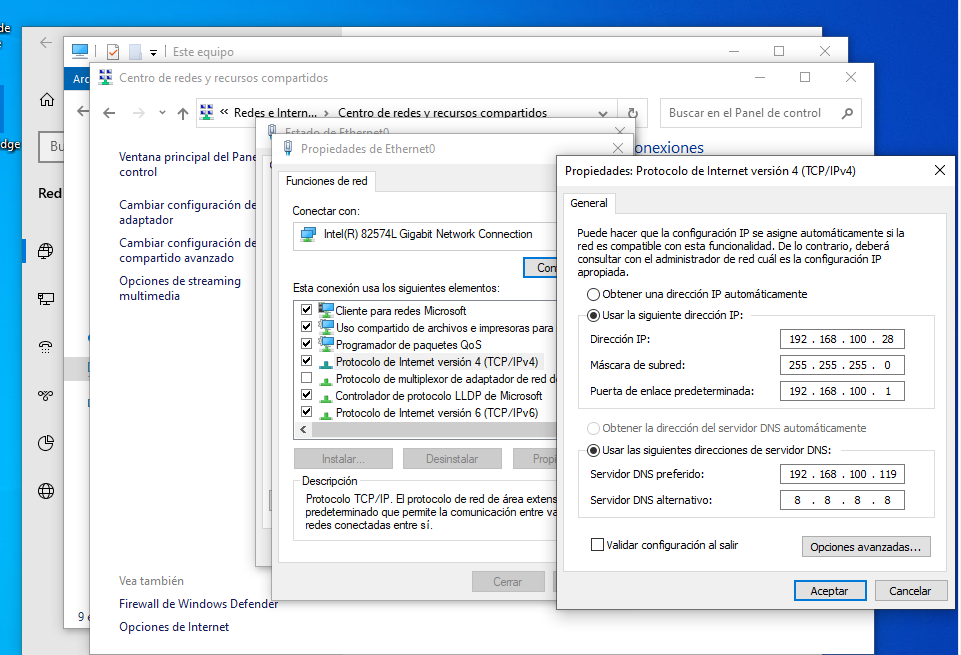
\includegraphics[width=0.8\textwidth]{config_red_win}
    \caption{Captura de administrador de dispositivos}\label{fig:confrwin}
  \end{figure}
  
\end{itemize}

\newpage{}
\paragraph{SAMBA AD DC}\ \\Añadir cliente al demonio
\begin{itemize}
\item Click derecho a equipo y \lstinline|propiedades/configuracion avanzada/Nombre de equipo/ boton cambiar...|
  \begin{figure}[H]
    \centering
    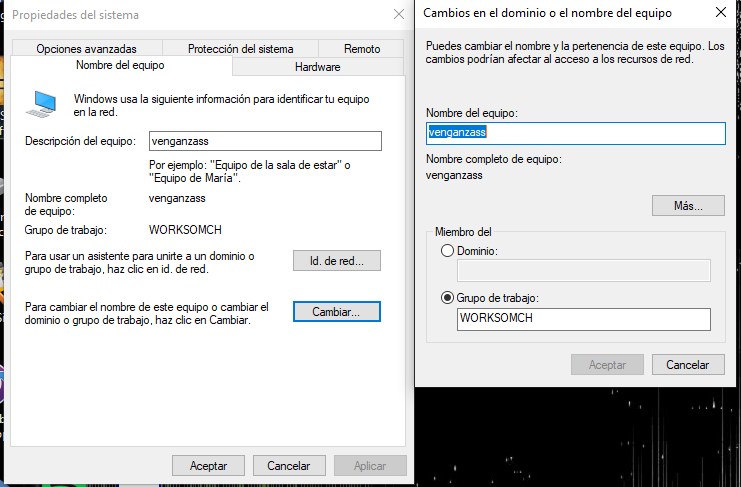
\includegraphics[width=0.8\textwidth]{config_cambiar}
    \caption{Configuracion del nombre del equipo}\label{fig:config_cambiar}
  \end{figure}
\newpage{}
  
\item En la seccion Miembro del seleccionar Dominio poner el dominio del servidor SAMBA que es \lstinline|srv.nis|
  \begin{figure}[H]
    \centering
    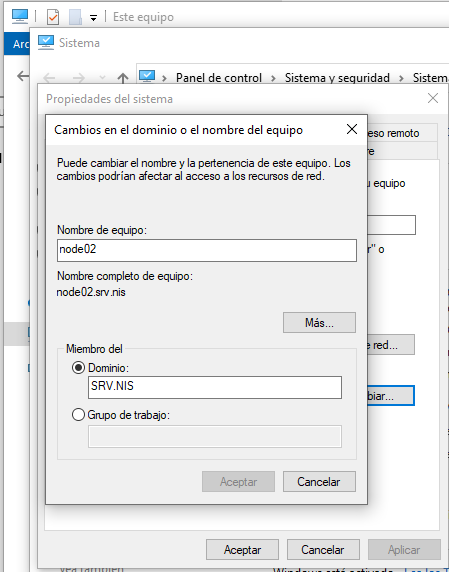
\includegraphics[width=0.8\textwidth]{config_cambiar_domi}
    \caption{Captura de asignacion de dominio}\label{fig:config_cambiar_domi}
  \end{figure}
  \newpage{}
\item Si sale un dialogo de inicio de sesion usar el usuario ``Administrator''
  y poner la contraseña proporcionada en la configuracion
\item Añadir el script \lstinline|drive.bat| a la carpeta de programas
  de inicio para automontar la unidad \lstinline|Z| al inicio de sesion de
  cada usuario.
  \begin{figure}[H]
    \centering
    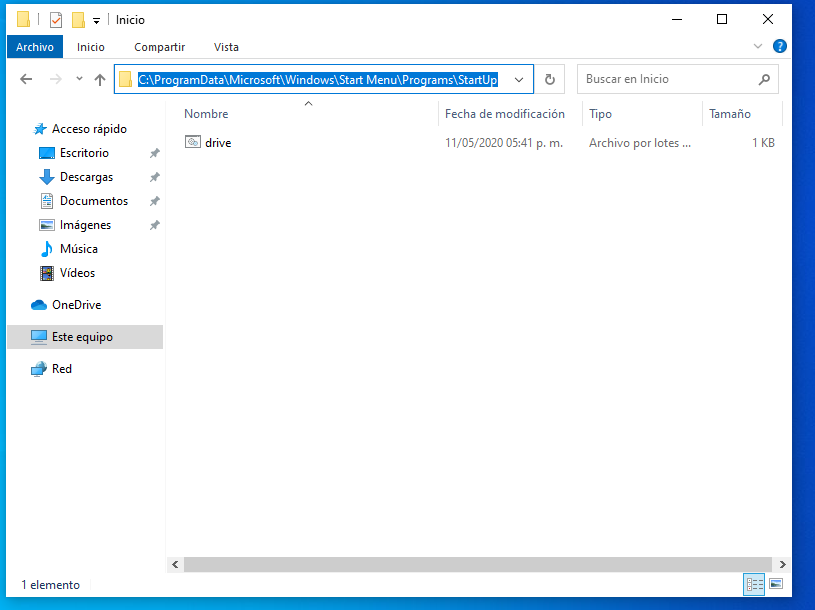
\includegraphics[width=0.8\textwidth]{menu_inicio}
    \caption{Captura de menu de inicio}\label{fig:menu_inicio}
  \end{figure}

  el contenido de este \lstinline|drive.bat| es el siguiente:

  \lstinputlisting[language=sh,label={list:drive},caption=Contenido de drive.bat]{../../configs/drive.bat}

\item Para adaptar a caso de uso diferente
  modificar \lstinline|\SRV.NIS| por el nombre de dominio.
  correspondiente.
\item Reiniciar equipo
    \newpage{}
\item Si todo sale bien debe poder iniciar sesion con los
  usuarios creados en el servidor SAMBA
  \begin{figure}[H]
    \centering
    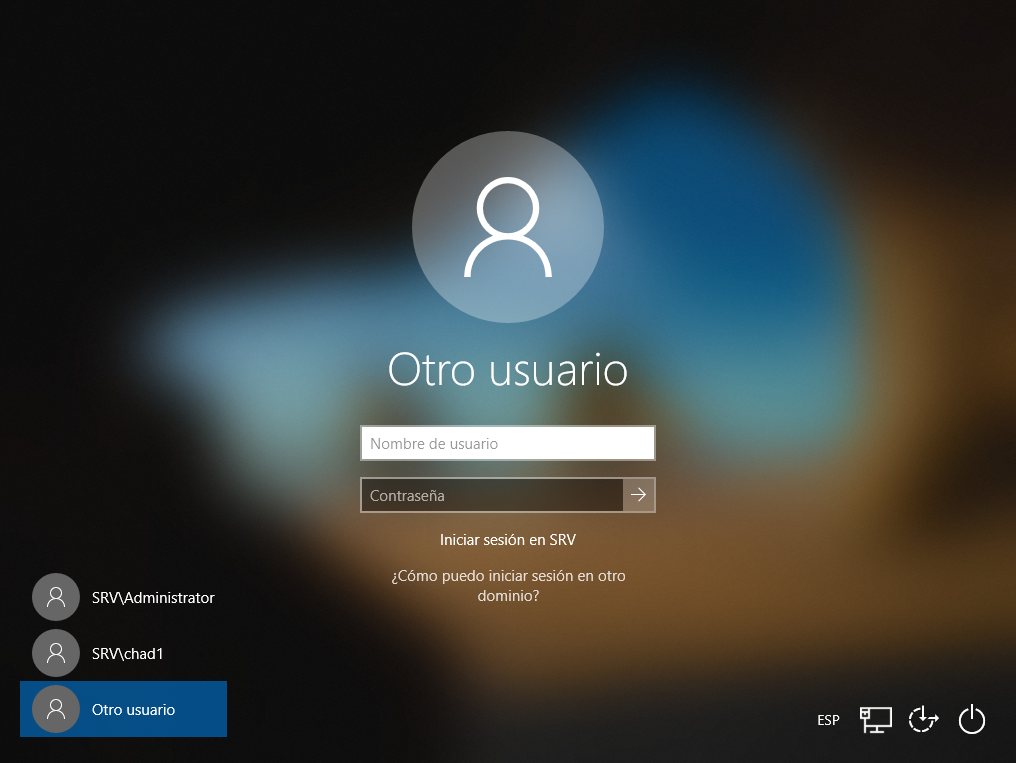
\includegraphics[width=0.8\textwidth]{inicio_sesion}
    \caption{Captura de inicio de sesion}\label{fig:inicio_sesion}
  \end{figure}
  \newpage{}
\item La unidad Z con la carpeta home del usuario debe montarse al
  inicio de cada sesion
  \begin{figure}[H]
    \centering
    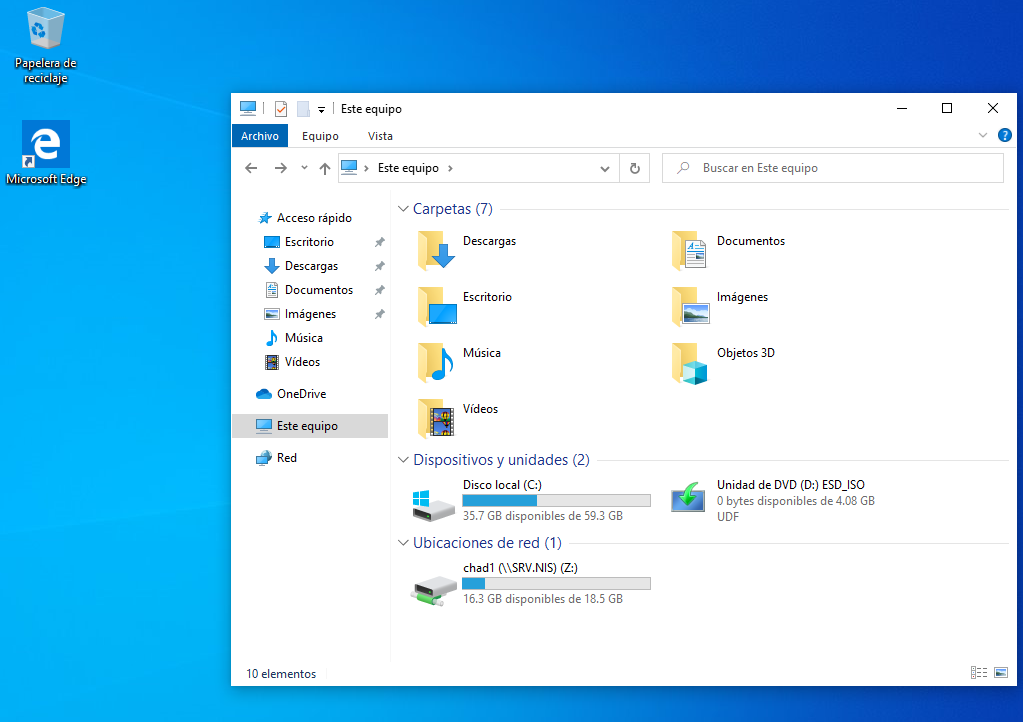
\includegraphics[width=0.8\textwidth]{samba_drive_z}
    \caption{Captura de inicio de sesion}\label{fig:samba_drive_z}
  \end{figure}

\end{itemize}






\end{document}
